\FloatBarrier
\section{Behavioral Cloning}
\label{sec::71_bc}
Behavioral cloning in itself is not always related to machine learning but poses one possible way of training a neural network in a supervised manner. The presented concept is easy to understand and got inspired by \cite{bojarski2016end}, where they used it for self-driving cars, and since having a car drive along the road is easier to achieve than having a robot walk around an environment, we will deal with the additional details later to focus on the main points for now. The proposed method utilizes the control loop, which was already introduced in figure \ref{fig::7_cl}. In order to then replace the human user by an artificial agent, we have a human user perform a desired behavior, and copy it. The required extended control loop is shown in figure \ref{fig::71_bc}.
\begin{figure}[h!]
	\centering
	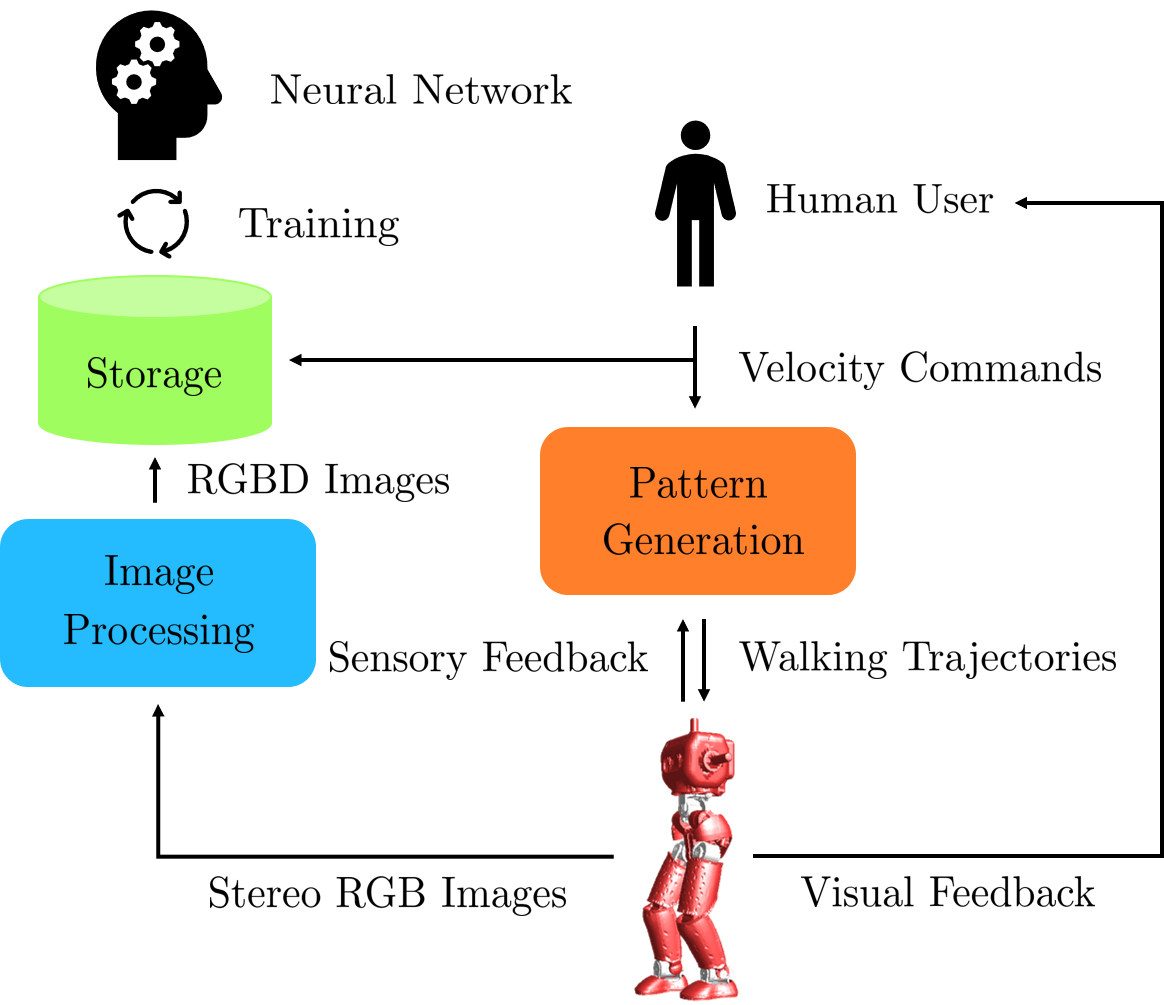
\includegraphics[scale=.5]{chapters/07_autonomous_high_level_control_of_the_walking_pattern_generator/img/behavioral_cloning.png}
	\caption{Pipeline for behavioral cloning. The neural network is trained on stored RGBD images, and corresponding velocity commands that are correlated by a timestamp}
	\label{fig::71_bc}
\end{figure}
It simply takes the velocity commands from the human user and stores it alongside RGBD images with a corresponding timestamp to some storage, where the RGBD images are obtained from stereo RGB images by an image processing step that is explained in section \ref{sec::3_ip}. The timestamp allows to correlate seen images to desired velocities afterward, which in turn enables an artificial agent to train on the stored data. For our purposes, the artificial agent is a neural network. An appropriately chosen network architecture will then enable us to learn the taught behavior and ultimately lets us replace the human user. This procedure relies on prior knowledge to achieve certain tasks, namely the stored data. It is therefore essential to assure that the sampled data, from which we want to learn a task, does not introduce any unwanted bias. That is, we need to take care of the distribution from which we sample in the first place. In principle, it is possible to learn any arbitrary behavior with this technique, but this requires not only good data, but also a vast amount of it. Other algorithms explore the state space on their own, and for which we could, for example, use the taught behavior as prior as well. These algorithms belong to the class of reinforcement learning methods, and we will have a look at a particular one in the next section.
\\\\ TODO
In the previous sections, we have learned about two different approaches to train neural nets on solving certain tasks. Although we came to understand that the complexity of the task to be solved correlates strongly with the amount of data at hand, there exist domains from which it is undeniably easier to do so. To equip a neural network with some prior knowledge by switching the domain may therefore not only be highly desirable but sometimes also needed if the amount or quality of data is not sufficient. One domain which is of special interest when it comes to interacting in a three-dimensional environment is a domain that represents depth information. If there are any, it may sometimes be possible to extract this kind of prior knowledge from a depth camera. As for this work, we need to rely on stereo cameras and powerful algorithms that allow us to compute depth images in real-time. The algorithm that helps us to do so, in terms of the extraction of weighted least squares disparity maps \cite{min2014fast}, will be presented in the following paragraph - Depth Map Extraction.
\\\\ TODO
Again, the first step within the deep learning pipeline is the image processing, as already introduced in section  \ref{sec::3_ip}. The camera calibration within this work was done using OpenCV \cite{opencv_library}. Exemplary code with which we did the depth map parameter tuning in section \ref{sec::102_dp}, can be found at the provided \href{https://github.com/mhubii/nmpc_pattern_generator/blob/master/src/tune_disp_map.cpp}{\underline{link}}. It relies on the rectification matrices $\bm{R}_i$, and the projection matrices $\bm{P}_i$ that got explained in section \ref{sec::3_ip}. YAML files store them inside of the io\_module folder of figure \ref{fig::62_folder}. They are highly dependent on the robot but will not change for Heicub over time, for why the future reader will be able to reuse them. As already explained in section \ref{sec::71_bc}, Heicub's recorded images and the corresponding velocities got stored inside of a folder. Locations to the image files, as well as the velocities, were then stored in a text file. For a faster prototyping, we then decided to implement the deep learning training pipeline within Python with PyTorch \cite{paszke2017automatic}, for which the routine can be found at the provided \href{https://github.com/mhubii/nmpc_pattern_generator/blob/master/libs/learning/python/train_rgbd.py}{\underline{link}}. The trained model got then converted to a just in time (JIT) script that loads into the executables in the src folder of figure \ref{fig::62_folder} via
\begin{minted}{cpp}
auto module = torch::jit::load(net_location);
\end{minted}
The code to convert a model, which got trained in Python, to C++, is part of the python folder and can be found at the following \href{https://github.com/mhubii/nmpc_pattern_generator/blob/master/libs/learning/python/python_to_cpp.py}{\underline{link}}. For Heicub, there was an additional step to be done, which is explained in section \ref{sec::8_co}, but given the camera images and depth maps are provided as \inlinecode{C++}{cv::Mat}, it is possible to convert them to a \inlinecode{C++}{torch::Tensor}, which can then be concatenated into a single RGBD tensor. We temporarily saved a sequence of these tensors, which enabled us to forward them through our long short-term memory based neural network, for which the architecture is given in figure \ref{fig::1111_unet}. For the behavioral augmentation, this can, for example, be seen at the provided \href{https://github.com/mhubii/nmpc_pattern_generator/blob/719fde0bb73925923de85cbf379c5523e075dfeb/src/behavioural_augmentation_real_robot_external_data.cpp#L625}{\underline{link}}. Once the neural network predicts a desired velocity for the pattern generation, one only has to convert the desired velocity back to an \inlinecode{C++}{Eigen::Vector3d}, which is the datatype that the pattern generation library works with. This velocity is then forwarded, just as described in section \ref{sec::63_us}, via the \inlinecode{}{NMPCPatternGenerator::SetVelocityReference} method, and a new iteration is executed. In the following section, we will explain how the developed pipelines can be used together with Heicub. It is therefore mainly required to implement the control loop of figure \ref{fig::7_cl}. 